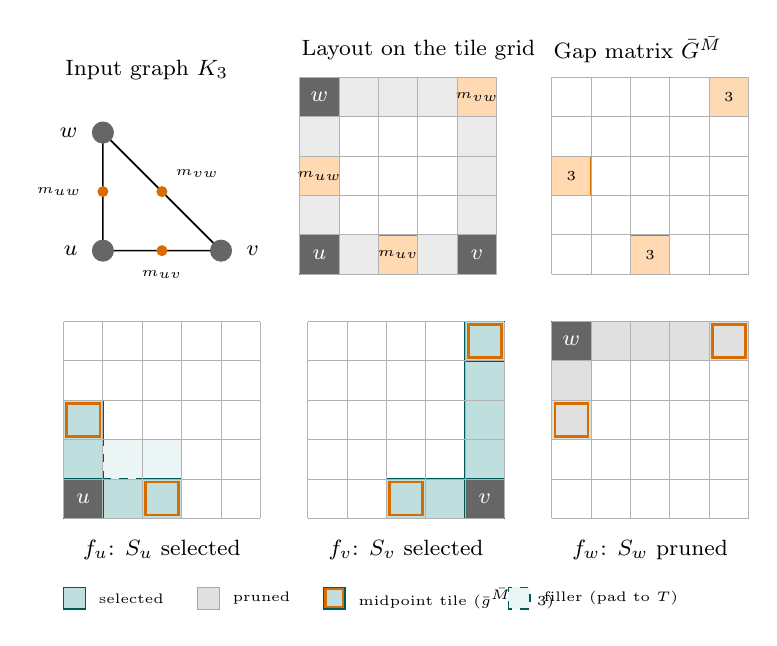
\begin{tikzpicture}[x=0.5cm,y=0.5cm]
  \tikzstyle{labelstyle}=[font=\footnotesize]
  \tikzstyle{tinylabel}=[font=\tiny]
  \tikzstyle{guidestyle}=[line width=0.3pt, draw=black!30]
  \tikzstyle{pathtile}=[draw=black!30, fill=black!8, line width=0.3pt]
  \tikzstyle{verttile}=[draw=black!70, fill=black!60, line width=0.3pt]
  \tikzstyle{keeptile}=[draw=teal!70!black, fill=teal!25, line width=0.45pt]
  \tikzstyle{droptile}=[draw=black!35, fill=black!12, line width=0.3pt]
  \tikzstyle{fillertile}=[draw=teal!70!black, dashed, fill=teal!8, line width=0.45pt]
  \tikzstyle{midtile}=[draw=orange!85!black, fill=orange!30, line width=0.45pt]
  \tikzstyle{midframe}=[draw=orange!85!black, fill=none, line width=0.9pt]

  % ---------- (a) input graph ----------
  \begin{scope}[shift={(1.0,6.8)}]
    \node[labelstyle, anchor=west] at (-1.2,4.6) {Input graph $K_3$};
    \draw[line width=0.6pt] (0,0) -- (3,0) -- (0,3) -- cycle;
    \fill[orange!85!black] (1.5,0) circle (0.14);
    \fill[orange!85!black] (0,1.5) circle (0.14);
    \fill[orange!85!black] (1.5,1.5) circle (0.14);
    \node[tinylabel, anchor=north] at (1.5,-0.25) {$m_{uv}$};
    \node[tinylabel, anchor=east] at (-0.3,1.5) {$m_{uw}$};
    \node[tinylabel, anchor=south west] at (1.6,1.6) {$m_{vw}$};
    \fill[black!60] (0,0) circle (0.28);
    \fill[black!60] (3,0) circle (0.28);
    \fill[black!60] (0,3) circle (0.28);
    \node[labelstyle, anchor=east] at (-0.4,0) {$u$};
    \node[labelstyle, anchor=west] at (3.4,0) {$v$};
    \node[labelstyle, anchor=east] at (-0.4,3) {$w$};
  \end{scope}

  % ---------- (b) orthogonal drawing on the tile grid ----------
  \begin{scope}[shift={(6.0,6.2)}]
    \node[labelstyle, anchor=west] at (-0.2,5.7) {Layout on the tile grid};
    % edge-path tiles
    \foreach \x/\y in {1/0,3/0,0/1,0/3,4/1,4/2,4/3,3/4,2/4,1/4} {
      \draw[pathtile] (\x,\y) rectangle ++(1,1);
    }
    % midpoint tiles
    \foreach \x/\y in {2/0,0/2,4/4} {
      \draw[midtile] (\x,\y) rectangle ++(1,1);
    }
    % vertex tiles
    \foreach \x/\y/\n in {0/0/u,4/0/v,0/4/w} {
      \draw[verttile] (\x,\y) rectangle ++(1,1);
      \node[labelstyle, text=white] at (\x+0.5,\y+0.5) {$\n$};
    }
    \node[tinylabel] at (2.5,0.5) {$m_{uv}$};
    \node[tinylabel] at (0.5,2.5) {$m_{uw}$};
    \node[tinylabel] at (4.5,4.5) {$m_{vw}$};
    \draw[guidestyle, step=1] (0,0) grid (5,5);
  \end{scope}

  % ---------- (c) gap matrix ----------
  \begin{scope}[shift={(12.4,6.2)}]
    \node[labelstyle, anchor=west] at (-0.2,5.7) {Gap matrix $\bar{G}^{\bar{M}}$};
    \foreach \x/\y in {2/0,0/2,4/4} {
      \draw[midtile] (\x,\y) rectangle ++(1,1);
      \node[tinylabel] at (\x+0.5,\y+0.5) {$3$};
    }
    \draw[guidestyle, step=1] (0,0) grid (5,5);
  \end{scope}

  % ---------- (d) one frame per vertex ----------
  % frame f_u : S_u selected (with filler to reach T = 7)
  \begin{scope}[shift={(0,0)}]
    \foreach \x/\y in {1/0,0/1} {
      \draw[keeptile] (\x,\y) rectangle ++(1,1);
    }
    \foreach \x/\y in {1/1,2/1} {
      \draw[fillertile] (\x,\y) rectangle ++(1,1);
    }
    \foreach \x/\y in {2/0,0/2} {
      \draw[keeptile] (\x,\y) rectangle ++(1,1);
      \draw[midframe] (\x+0.08,\y+0.08) rectangle ++(0.84,0.84);
    }
    \draw[verttile] (0,0) rectangle ++(1,1);
    \node[labelstyle, text=white] at (0.5,0.5) {$u$};
    \draw[guidestyle, step=1] (0,0) grid (5,5);
    \node[labelstyle] at (2.5,-0.8) {$f_u$: $S_u$ selected};
  \end{scope}

  % frame f_v : S_v selected
  \begin{scope}[shift={(6.2,0)}]
    \foreach \x/\y in {3/0,4/1,4/2,4/3} {
      \draw[keeptile] (\x,\y) rectangle ++(1,1);
    }
    \foreach \x/\y in {2/0,4/4} {
      \draw[keeptile] (\x,\y) rectangle ++(1,1);
      \draw[midframe] (\x+0.08,\y+0.08) rectangle ++(0.84,0.84);
    }
    \draw[verttile] (4,0) rectangle ++(1,1);
    \node[labelstyle, text=white] at (4.5,0.5) {$v$};
    \draw[guidestyle, step=1] (0,0) grid (5,5);
    \node[labelstyle] at (2.5,-0.8) {$f_v$: $S_v$ selected};
  \end{scope}

  % frame f_w : S_w pruned
  \begin{scope}[shift={(12.4,0)}]
    \foreach \x/\y in {0/3,1/4,2/4,3/4} {
      \draw[droptile] (\x,\y) rectangle ++(1,1);
    }
    \foreach \x/\y in {0/2,4/4} {
      \draw[droptile] (\x,\y) rectangle ++(1,1);
      \draw[midframe] (\x+0.08,\y+0.08) rectangle ++(0.84,0.84);
    }
    \draw[verttile] (0,4) rectangle ++(1,1);
    \node[labelstyle, text=white] at (0.5,4.5) {$w$};
    \draw[guidestyle, step=1] (0,0) grid (5,5);
    \node[labelstyle] at (2.5,-0.8) {$f_w$: $S_w$ pruned};
  \end{scope}

  % ---------- legend ----------
  \begin{scope}[shift={(0,-2.3)}]
    \draw[keeptile] (0,0) rectangle ++(0.55,0.55);
    \node[tinylabel, anchor=west] at (0.65,0.27) {selected};
    \draw[droptile] (3.4,0) rectangle ++(0.55,0.55);
    \node[tinylabel, anchor=west] at (4.05,0.27) {pruned};
    \draw[keeptile] (6.6,0) rectangle ++(0.55,0.55);
    \draw[midframe] (6.65,0.05) rectangle ++(0.45,0.45);
    \node[tinylabel, anchor=west] at (7.25,0.27) {midpoint tile ($\bar{g}^{\bar{M}} = 3$)};
    \draw[fillertile] (11.3,0) rectangle ++(0.55,0.55);
    \node[tinylabel, anchor=west] at (11.95,0.27) {filler (pad to $T$)};
  \end{scope}
\end{tikzpicture}
